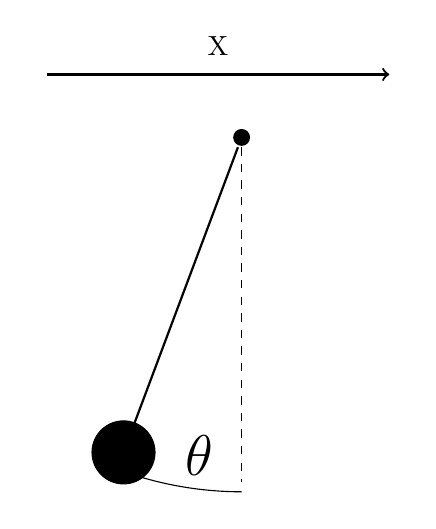
\begin{tikzpicture}

\node (p1) at (-1,1) {};
\node (p2) at (-2.5,-3) {};
\node (p3) at (-1,-3.5) {};
\draw [fill] (p1) circle [radius=0.1];
\draw [fill] (p2) circle [radius=0.4];
\draw [thick] (p1) -- (p2);
\draw [dashed] (p1) -- (p3);


\draw (-2.65656,-3.183994) arc (-111.599995:-90:4.5) node [midway,above right] {\fontsize{20}{20}$\theta$};
\node (i) at (-3.6,1.8) {};
\node (f) at (1,1.8) {};
\draw [->, thick] (i) -- (f) node [black, midway, above=3] {X};
\end{tikzpicture}